% Auto-generated by src/make_paper_figures.py; do not edit by hand.
\begin{figure}[t]
\centering
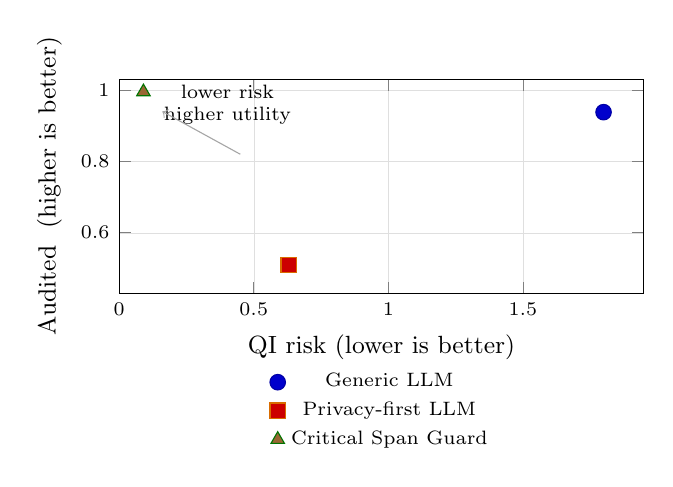
\begin{tikzpicture}
\begin{axis}[
  width=0.68\linewidth,
  height=4.3cm,
  xmin=0,
  xmax=1.95,
  ymin=0.43,
  ymax=1.03,
  xlabel={QI risk (lower is better)},
  ylabel={Audited \tcfr{} (higher is better)},
  grid=both,
  grid style={line width=.1pt, draw=gray!25},
  tick label style={font=\scriptsize},
  label style={font=\small},
  legend style={font=\scriptsize, draw=none, fill=none, at={(0.5,-0.32)}, anchor=north, legend columns=1},
  clip=false,
]
\addplot+[only marks, mark=*, mark size=2.8pt, color=blue!65!black] coordinates {(1.800,0.938)};
\addlegendentry{Generic LLM}
\addplot+[only marks, mark=square*, mark size=2.8pt, color=orange!85!black] coordinates {(0.630,0.510)};
\addlegendentry{Privacy-first LLM}
\addplot+[only marks, mark=triangle*, mark size=2.8pt, color=green!45!black] coordinates {(0.090,0.995)};
\addlegendentry{Critical Span Guard}
\node[font=\scriptsize, align=center, anchor=west] at (axis cs:0.13,0.96) {lower risk\\higher utility};
\draw[->, gray!70] (axis cs:0.45,0.82) -- (axis cs:0.16,0.94);
\end{axis}
\end{tikzpicture}
\caption{Privacy--utility frontier for the 100-example non-oracle LLM run. \method{} is closest to the upper-left target region: lower measured quasi-identifier risk and higher audited task-critical fact retention.}
\label{fig:frontier}
\end{figure}
